Moving from all we learnt in the previous chapters, this one will discuss the implementation of the linpack benchmark and the implementation of a $\pi$ approximation, using an easily parallelizable algorithm. It will be discussed the limits set by the granularity of a program and the speedup obtained with the \glspl{eCore} versus the host.

\section{Linpack}

The purpose of this section is to optimize the c linpack implementation with the help of the \gls{epiphany} side and its 16 cores. We will be optimizing a function computing a constant times a vector plus a vector :
\begin{lstlisting}
for (i = 0;i < n; i++) {
  dy[i] = dy[i] + da*dx[i];
}
\end{lstlisting}

We will attempt to take the model (see fig \ref{fig flow general}) discussed in the previous chapter and improve it, especially the \gls{epiphany} part. The aim is to beat 120MFlop obtained by the host part only.

The first results obtained with the help of the \gls{epiphany} side are much worse than those obtained with the host part only.

To communicate with the \gls{epiphany} side, we need to use shared buffer as shown in section \ref{ex3}. In our case - constant times a vector plus a vector - it implies declaring and using 3 shared buffers :

\begin{itemize}
  \item Vector[n], array of size n
  \item Vector[n], array of size n
  \item C, a constant
\end{itemize}

Those buffers are to be initialized each time the function is called :

\begin{lstlisting}
status = e_write(&shareddy,  0, 0, 0x0, dy, n*sizeof(REAL));
printf("[info] Status of shareddy writing: %i\n", status);
status = e_write(&sharedda, 0, 0, 0x0, &da,   sizeof(REAL));
printf("[info] Status of sharedda writing: %i\n", status);
status = e_write(&shareddx, 0, 0, 0x0, dx, n*sizeof(REAL));
printf("[info] Status of shareddx writing: %i\n", status);
\end{lstlisting}

Unfortunately for us, we measured that the only fact of initializing those buffers decreases performances by more than 5 times comparing to the host only implementation. Meaning that doing better than the host implementation is impossible with shared buffers. Figure \ref{graph flops decrease} shows metrics of KFlops measured with only the host side and with the buffer declaration.

As shown previously in figure \ref{code profilling}, the method we are working on is called 1060694 times. Hence, calling so often the buffers initialization is not reasonable and will never make better results than the host implementation. In a more general way, our program offers high concurrency and should have a coarse granularity to avoid excessive concurrency \cite{pie}. But the way we sent small operations to the \gls{epiphany} offers too much granularity by it's executing time and the number of time it is called comparing to the total executing time. Meaning that, in this particular case, transfer times are too important. In our case, we will not raise granularity since it would require changing the way linpack uses \code{daxpy}.

\begin{figure}[h!]
\centering
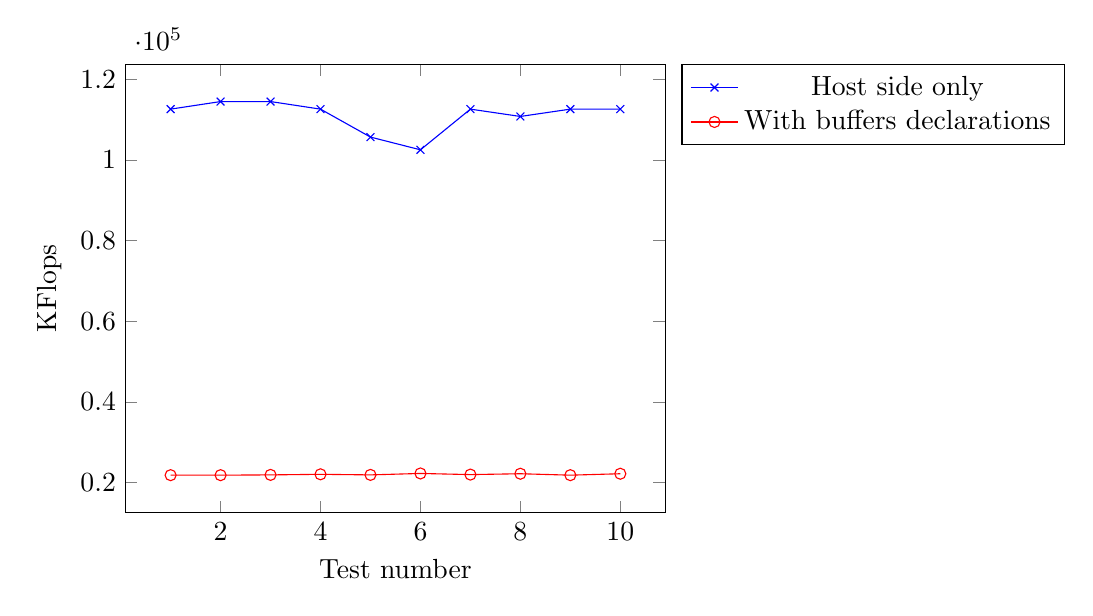
\begin{tikzpicture}
	\begin{axis}[
		xlabel=Test number,
		ylabel=KFlops,
		legend pos=outer north east]
	\addplot[color=blue,mark=x] coordinates {
		(1,112568)
		(2,114444)
		(3,114444)
		(4,112568)
		(5,105641)
		(6,102488)
		(7,112568)
		(8,110753)
		(9,112568)
		(10,112568)
	};
	\addlegendentry{Host side only}
	\addplot[color=red, mark=o] coordinates {
		(1,21868)
		(2,21868)
		(3,21938)
		(4,22079)
		(5,21938)
		(6,22294)
		(7,22009)
		(8,22222)
		(9,21868)
		(10,22222)
	};
	\addlegendentry{With buffers declarations}
	\end{axis}
\end{tikzpicture}
\caption{Measure of KFlops running c linpack on the host and with the shared buffers declaration. The host side is around 110MFlops, with shared buffer declaration arround 21MFlops.}
\label{graph flops decrease}
\end{figure}

Moving from this observation, we have three options :

\begin{itemize}
  \item Finding a way not to to initialize buffers in the function
  \item Finding a way not to use shared buffers
  \item Trying to raise the granularity by changing the implementation
\end{itemize}

Trying to initialize buffers outside the \code{daxpy} method is not possible since each time the method is called, we use new data to be shared. We could bypass the need of using shared buffers by exploiting the \glspl{eCore}' local memory, but this option would make the implementation more complex and be limited by the \glspl{eCore}' local memory size.

Finally, as said before, we would need to change the architecture of the linpack implementation to find a way of raising the granularity.

\section{$\pi$ approximation}

This section will be focused on implementing a concurrent program that will be approaching the PI value using machin-like formula (\ref{eq:machin-like}). The advantage of this formula is to be highly parallelizable. Because it is an infinite sum, we can easily distribute part of the sum across cores. 

\begin{equation}
	\pi = 4 \cdot \sum_{n=1}^{\infty} \frac{(-1)^n}{2n + 1}
	\label{eq:machin-like}
\end{equation}

We will be working on implementing an host only version of the PI approximation using machin-like formula, and an \gls{epiphany} version, using the \glspl{eCore}. The formula will be implemented as a loop calling a function which computes part of the sum. That function will then be distributed among \glspl{eCore}. The main loop size will represent the main number of iterations, and the part size of the sum the function will compute will be called the sub-iterations number.

Figure \ref{fig machin-like} is a representation of the sub and main iterations. The total number of iterations is given by the number of main iterations times the number of sub iterations. The sub iterations will be distributed among \glspl{eCore}.

\begin{figure}[h!]
\centering
\includegraphics[width=.5\textwidth]{machin-like.pdf}
\caption{Representation of the machin-like implementation using sub and main iterations}
\label{fig machin-like}
\end{figure}

The code remains simple, it is a loop calling $N$ times a function which runs $n$ iterations. Hence, it is computing the sum for $N \cdot n$ iterations. The code for the host only implementation is quite straightforward :

\begin{lstlisting}
for(i = 0; i < main_iteration; i++) {
  res = res + f(i);
}

float f(unsigned x) {
  float res = 0;
  unsigned a = x * sub_iteration;
  unsigned b = a + sub_iteration;
  for(; a < b; a++) {
    res += pow(-1,a) / (2*a + 1);
  }
  return res;
}
\end{lstlisting}

To adapt our code for the \gls{epiphany}, we moved the function computing the sub iterations to the \glspl{eCore}' program. We then made the host managing \glspl{eCore} to compute the sub iterations, getting results and making the addition of all \glspl{eCore} results. We used the same concept spoken in section \ref{benchmark}, but using only local \glspl{eCore}' memory to set instruction and getting results.

The first measures we made was comparing execution times between the host implementation and the \gls{epiphany} one. We also wanted to know the impact of the number of main iterations with respect to the number of sub iterations. What we did was executing our program inside two loops modifying the number of main and sub iterations. We did the same operations for the host only implementation and the \gls{epiphany} one. We then plotted the results in a 3D graph showing the main number of iterations, the sub number of iterations and the execution time.

Figures \ref{fig measures pi1} and \ref{fig measures pi2} show the 3D graph obtained after plotting our results. What we can note is that the variance of the main number of iterations and sub iterations for the same total number of iterations does not affect the execution time. Figure \ref{fig measures pi1} compares the two implementations, the host one is on top. We see that the \gls{epiphany} implementation is about two times faster. Figure \ref{fig measures pi3} gives a better representation of the performance, giving, for the two implementations, the total number of iteration with the execution time. Figure \ref{fig measures pi2} is the top view of the 3D graph for each implementations. We plotted on top of it curves showing values for $N*n$ (number of iterations times number of sub iterations is constant), showing that for the same number of iterations, the variance of $N$ and $n$ gives the same execution time.

\begin{figure}[h!]
\centering
\noindent\makebox[\textwidth]{\includegraphics[width=.8\textwidth]{measures/both.pdf}}
\caption{Comparing time execution of host only and \gls{epiphany} computation of pi using machin-like method}
\label{fig measures pi1}
\end{figure}

\begin{figure}
  \begin{subfigure}{.5\textwidth}
  \centering
  \noindent\makebox[\textwidth]{\includegraphics[width=1\linewidth]{measures/stats-archive-top.pdf}}
  \end{subfigure}
  \begin{subfigure}{.5\textwidth}
  \centering
  \noindent\makebox[\textwidth]{\includegraphics[width=1\linewidth]{measures/stats-archive-top.pdf}}
  \end{subfigure}
\caption{Top view of time execution with respect to iterations number}
\label{fig measures pi3}
\end{figure}

\begin{figure}[h!]
\centering
\noindent\makebox[\textwidth]{\includegraphics[width=.8\textwidth,page=2]{measures/both.pdf}}
\caption{Comparing time execution of host only and \gls{epiphany} computation of pi using machin-like method}
\label{fig measures pi2}
\end{figure}

Our second measure will be the speedup obtained by using the \gls{epiphany} comparing to using only the host with its ARM-A9 processor. For the test, we will need a constant number of iterations, $M$, which corresponds to $M = N \cdot n$ ($N$ is the number main of iterations, $n$ the number of sub iterations). To compute the speedup, we will run our program with different number of cores. Then, we will compare the execution time when using one core with the time obtained with one to sixteen cores (\glspl{eCore}).

To keep the same number of iterations, we will use those formulas :

\begin{align*}
	M = N \cdot n \\
	n = \frac{M}{k \cdot nb_{cores}}\\
	N = k \cdot nb_{cores}
\end{align*}

with $M$ the total number of iterations, $N$ the number of main iterations, $n$ the number of sub iterations, $nb_{cores}$ the number of cores and $k$ a factor dividing the number of sub iterations. In our measures, we chose a constant $M$ which is divisible by the total number of cores and a constant k. We then ran the program making the number of cores varying from 1 to 16 (the total number of \glspl{eCore}). With the time obtained, we used it to divide the reference time, taken as the time used by the host only (hence one core). This time is taken as the \textit{time to beat}.

Figure \ref{fig speedup} shows the speedup of the \gls{epiphany} according to the host. We see that to obtain the same performance of the host, we need to use seven \glspl{eCore} and the maximum speedup using all the \glspl{eCore} gives an execution time 2.24 times faster than the host only.

\begin{figure}[h!]
\centering
\noindent\makebox[\textwidth]{\includegraphics[width=.8\textwidth,page=1]{measures/speedup.pdf}}
\caption{Speed up results, the reference time is the host}
\label{fig speedup}
\end{figure}

In section \ref{architecture}, we saw that the host side runs an ARM-A9 at 866MHz, while each \gls{eCore} runs at 1GHz. So even using a single \gls{eCore} against the host should be faster, but our measures shows that a single \gls{eCore} is seven times slower than the host. In fact, the documentation provided by Adapteva\cite{epiphanyArch}\cite{parallellamanual} tells us that the 1GHz stands for the operating frequency of the \glspl{eCore}' mesh network. But, in out test, we didn't use that mesh network at all. Because each jobs was dispatched from the host to each individual \gls{eCore}, we didn't benefit from the mesh network provided by the \gls{epiphany} architecture. Hence, our results are reasonable given the fact that we didn't use all the capacities of the \gls{epiphany} architecture.

Taking a single \gls{eCore} as the reference time gives a linear growing speedup following nearly the ideal case. The figure \ref{fig speedup2} shows that our problem is well distributed among \glspl{eCore} and that the parallel portion of our program is near 100\%. In this case, transfer times are negligible. 

\begin{figure}[h!]
\centering
\noindent\makebox[\textwidth]{\includegraphics[width=.8\textwidth,page=2]{measures/speedup.pdf}}
\caption{Speed up results, the reference time is one \gls{eCore}}
\label{fig speedup2}
\end{figure}

%\begin{figure}[h!]
%\centering
%\noindent\makebox[\textwidth]{\includegraphics[width=.8\textwidth,page=3]{measures/speedup.pdf}}
%\caption{Efficiency based on speedup}
%\label{fig speedup}
%\end{figure}

\section{Conclusion}

In this chapter, we tried to improve the linpack implementation without any success. What we learnt from that was an important fact: concurrent programming cannot improve a program at a too small granularity level depending on its transfer times. In our case, communication times was far over the execution time of the code we wanted to improve. We would need to re-think the implementation of the linpack program so as to raise the granularity.

Moving from the linpack, we took this opportunity to implement an approximation of $\pi$ that would offer an easy concurrent implementation. We found out that, for this problem, the host is seven times faster than a single \gls{eCore}, and using sixteen \gls{eCore} against the host is only 2.24 times faster. That result is far bellow what we could expect. One explanation would be the way jobs are distributed, without using the \gls{epiphany} mesh network at all. The speedup taking a single \gls{eCore} as a reference time grows linearly, nearly following the ideal case. This show us that our problem is well distributed and communication times doesn't affect much the speed. It would have been interesting to test with more than sixteen cores, for example using many parallella boards connected together.